\documentclass[conference]{IEEEtran}

\makeatletter
\def\ps@headings{%
\def\@oddhead{\mbox{}\scriptsize\rightmark \hfil \thepage}%
\def\@evenhead{\scriptsize\thepage \hfil \leftmark\mbox{}}%
\def\@oddfoot{}%
\def\@evenfoot{}}
\makeatother
\pagestyle{headings}

%\documentclass[preprint,10pt,nocopyrightspace]{sigplan-proc-varsize}
%\documentclass[preprint,10pt]{acm_proc_article-sp}
%!PN, old LaTeX209 font commands, replaced by the new ones
% keeping just this one
%\def\tenrm{\fontsize{10}{12}\normalfont\rmfamily\selectfont}
%\def\BibTeX\left\{ \rmfamily B\kern-.05em{\scshape i\kern-.025em b}\kern-.08em \TeX}}
\usepackage{epsfig}
\usepackage{verbatim}
\usepackage{amsmath}
\usepackage{amsfonts}
\usepackage{framed}
\usepackage{multirow}
\usepackage{subfigure}
\newtheorem{theorem}{Theorem}
\newtheorem{proposition}{Proposition}
\newtheorem{lemma}{Lemma}
\newtheorem{definition}{Definition}


\begin{document}
\title{A Distributed Android Security Framework}
%\author{
%    Benjamin E. Andow and Haodong Wang\\
%    Computer Science Department\\
%    Cleveland State University\\
%    Cleveland, OH 44115, USA
%}


\maketitle
\begin{abstract}

%As mobile devices continue to become increasingly ubiquitous in
%society, the demand for incorporating their use in the healthcare
%industry is concurrently rising.  However, 
The current security
models on mobile devices do not provide the level of
protection that is needed for the devices to handle sensitive
data, such as protected healthcare information.  In this paper, we
introduce a Distributed Android Security Framework (DASF). DASF is
a custom security framework for Android-based mobile devices that
allows dynamic security policies to be enforced on an application's
privileges and sensitive data.  DASF allows a server to dynamically
impose the security policies by utilizing an application-layer
message protocol that is implemented in the system.  The security
policies enforced by DASF enables the system-wide
privilege restrictions to be enforced on untrustworthy
applications and sensitive data.  Ultimately, DASF
allows the organization that issues
the mobile devices to dynamically dictate the security
policies enforced by the system and retain control
of the sensitive data that they send to the device.

\end{abstract}

\section{Introduction}

The incorporation of mobile devices in the healthcare industry can prove to be
another beneficial tool for medical professionals, as doctors and nurses
frequently communicate with each other to provide a diagnosis and treatment.
While the appeal of modern communication through mobile devices, e.g.,
smartphones or tablets, has reached almost every other industry, the following
observations witness the status of mobile devices in healthcare industry.
First, a significant number of physicians and nurses are still relying on
traditional clinical communication equipment, including pagers, phones and fax
machine, yet a last generation wireless communication technology. Second, even
though as many as 81\% healthcare professionals own and use the smartphones
themselves every day~\cite{manhattan}, their devices either are not integrated
into the healthcare communication system (so that pagers are still needed), or
cannot be trusted as the system components due to lacking of the security
mechanism compliant to Health Insurance Portability and Accountability Act
(HIPAA). It is reported \cite{mdnews} that lost, stolen, and non-HIPAA
compliant healthcare mobile applications are blamed for protected health
information (PHI) breach on electronic health record (EHR) systems. 

To take advantage of modern communication means supported by the mobile
devices, such as multimedia (text, image, and video) messaging and
conferencing, and fully employ the emerging technologies in healthcare industry
with HIPAA compliance, a system-wide security safeguard must be included to
defend against the potential security breaches. Checking the HIPAA privacy
rule~\cite{hipaarule}, we consider the following three security challenges for
the deployment of the mobile devices in healthcare industry.

\begin{itemize}
\item \textit{Network security:} The user authentication and data
  encryption schemes must be robust to protect PHI transmitted in the
  communication channel and defend against various security attacks.
\item \textit{Sensitive data flow confinement:} The service
  administrator should be able to control the propagation of the
  sensitive data and, if necessary, revoke the access to protected
  data that is sent to the mobile devices. For example, the healthcare
  organization should prevent PHI from being saved to the devices
  (e.g., saving a medical record as a file) or being forwarded to
  another device.
\item \textit{Dynamic security demands and fine-grained access control
  policies:} Access control policies should be flexible enough to meet
  the dynamic security demands in the various scenarios that the
  mobile devices are utilized. For example, the service administrator
  may want to dynamically enforce system-wide access control policies
  on the mobile devices to allow the organizations to dictate their
  own security policies.  
%\item \textit{PHI propagation control and revocation:} Healthcare
%  organizations should be able to control the propagation of the PHI
%  and revoke access to the PHI that is sent to the mobile device. For
%  example, the healthcare organization should be able to prevent PHI
%  from being saved to the device (e.g., saving a medical record as a
%  file on the device) or being forwarded to another device (e.g., sending a
%  medical record to another device). 
\end{itemize}
\begin{comment}
While the network security can be guarded by existing security
protocols, e.g., TLS/SSL, there is a non-trivial technical hurdle to
address the latter two challenges to protect the data privacy.
This work focuses on dynamic security provisioning and sensitive data
propagation control.   
%In this work, we select the Android
%mobile operating system as the platform to develop our custom security
%platform. 
%To address the aforementioned security challenges and meet the
%requirements of the HIPAA regulations, we select the Android mobile
%operating system as the platform to develop our custom security
%framework. However, the existing security model on the Android
%platform fails to address the security challenges. In particular,
The current mobile operating systems, e.g., Android, only support
%Android's current security model supports 
static installation-time privilege control and do not support the
dynamic restriction of previously granted privileges. Furthermore,
their security model also does not include a mechanism to control the
propagation and revocation of sensitive data on the device. One may
note that the above data protection can be addressed in the
application level by carefully designing and developing a
privacy-preserving application. Unfortunately, the application
level protection can be easily compromised due to the nature of the
mobile devices and the limitations of the mobile operating
systems. First, a stolen or lost device would give the adversary a
total access of its stored data (e.g., by sideloading a malicious
application that performs a full memory dump).  Second, a misbehaving
user may also launch the above attack or simply acquires the system
privilege (e.g., by rooting the device) to gain free access to the
data stored in the memory. Therefore, we argue that a standalone
mobile operating system is lacking the security
measures that can defend against various security attacks toward the
sensitive data. In this work, we propose a novel security design
concept for mobile operating system: a distributed security
framework (DSF).  DSF is based on a centralized (e.g., a cloud or a
server) security system, and pushes the security boundary along the
way to the mobile devices that include the mobile operating system
(e.g., Android). In our design, user devices are tightly 
coupled with the system server so that DSF makes sure all system
activities on the device side are compliant with the system security
policies. The loss of coupling between the device and the server,
including stolen, lost and system rooting, is considered as the
security attack that results in the security countermeasures, e.g.,
remote wipe-out. 
\end{comment}
This paper uses the healthcare communication application as a platform to
demonstrate the design and development of a Distributed Android Security
Framework (DASF), a customized security framework for Android-based mobile
operating systems designed to provide dynamic privilege restrictions on
applications and security policies on sensitive data on the device. The
coupling between the Android and a server is achieved by using secure
heart-beat messages through a system security channel established during
installation time.  In addition, DASF includes an application-layer networking
protocol (in regard to the OSI model) that allows the organization (e.g.,
hospital, clinic, etc.) to dictate their own security policies on the device
and on data sent to the device. DASF allows an application's access privileges
to be flexibly set up upon invocation and adjusted on-the-fly to meet the
various security needs when dealing with sensitive information. In mobile
devices that install DASF, the organization ultimately controls the security
policies that the system enforces on the user's device and on the sensitive
data that applications receive.

\begin{comment}
Therefore, the contributions that this paper provides are as
follows.  First, this paper provides a security policy
for dynamic system-wide privilege restrictions to be
enforced on applications.  Second, this paper also provides
a security policy that can be enforced on sensitive data.
The aforementioned security policies can either be utilized
by a server communicating with the mobile device or 
by a developer who is creating an application.
\end{comment}

%Our contributions in this paper can be summarized as follows. First,
%we use the medical communication system as an example to study the
%security problems and the HIPAA compliance issues caused by the
%mobile devices.  Second,
%we design a distributed Android security framework that not only
%provides dynamic system-wide security provisioning, but also protects
%the privacy of the received sensitive data and therefore defeats
%the PHI breach on mobile devices.  Third, we implement
%a prototype Android-based medical communication system and deploy our
%proposed security framework.  Our evaluation shows DASF is capable of
%defeating a variety of security attacks while only imposing a reasonable
%system overhead.

This paper makes the following contributions:
\begin{itemize}
	\item We study the security problems and HIPAA compliance issues
	caused by mobile devices, using a medical communication system as an example.
	\item We design a distributed Android security framework that not only
	provides dynamic system-wide security provisioning, but also protects
	the privacy of the received sensitive data, and therefore protects against PHI
	breaches on mobile devices.
	\item We implement a prototype Android-based medical communication
	system and deploy our proposed security framework.  Our evaluation shows DASF
	is capable of defeating a variety of security attacks while imposing a
	reasonable system overhead.
\end{itemize}

The remainder of this paper proceeds as follows. Section II discusses our
threat model and security assumptions. Section III formalizes the model of our
security framework. Section IV discusses our prototype's implementation.
Section V evaluates the security and performance of our prototype.  Section VI
discusses relevant related works. Finally, Section VII concludes.


\section{Threat Model and Security Assumptions}
\begin{comment}
This work focuses on the security challenges of enforcing security
policies on sensitive data sent to Android-based mobile devices and
enforcing dynamic privilege restrictions.
%Moreover, this work is focused on providing the security 
%guarantees at the system-level rather than at the application-level.
Thus, the security policies of the server and database management
system are out of scope of this study. And we assume that the data is
protected in the server (or cloud) and the database management system
by the appropriate security measures. Furthermore, we assume that the
server ensures that the communication channel between the server and
the application running on the mobile device is secure (e.g., SSL) and
each individual involved in the communication has his/her security
credentials (including digital certificates, public and private key,
etc.) distributed through an out-of-band security channel.  
\end{comment}
We assume that the Android OS, which includes the Linux kernel and Android's
system services (e.g., Activity Manager Service, Package Manager Service), is
trusted.
%We assume that an adversary may have physical access to the
%device, and can capture stored data and try to recover the sensitive data by
%all possible means.
We assume that all third-party Android applications installed on the mobile
devices (including \textit{medical applications}) are untrusted and may launch
attacks to try to gather sensitive information. However, we assume that these
third-party applications do not have root privileges, and do not collude with
other apps (e.g., covert channels).  Since the Android platform that we
augmented with DASF is transparent to application packages, malicious
applications may be installed and attempt to steal sensitive data from the
device or the environment. We assume the communication parties are
“semi-trusted”. That is, the user may misbehave by themselves (e.g., trying to
save or forward a patient's MRI image without proper authorization), but does
not conspire with the server. 

%Mobile devices are not trusted. Once the mobile device is lost or
%stolen, the adversaries can capture stored data and may try all
%possible means to recover the sensitive data.
%Further, all other third
%party Android applications installed on the mobile devices (including
%\textit{medical applications}) are not trusted and may launch attacks
%to try to gather sensitive information. Since the Android platform that we
%augmented with DASF is transparent to application packages, malicious
%applications may be installed and attempt to steal sensitive data from the
%device or the environment. We assume the communication parties are
%“semi-trusted”. That is, the user may misbehave by themselves (e.g., trying to
%save or forward a patient's MRI image without proper authorization) but do not
%conspire with the server. 

Therefore, we consider the following four different types of security
threats for which the system must provide protection. 

\begin{itemize}
\item \textit{Legitimate user misbehavior:} The system must prevent legitimate
users from manually attempting to save or forward sensitive information.
\item \textit{Malicious users:} The system must prevent sensitive information
from being recovered from the device if it is lost or stolen.
\item \textit{Application misbehavior:} The system must prevent legitimate
applications from attempting to save or forward sensitive information that is
not authorized by the organization's policies. For example, it is typical to
write an image to a file when it is received rather than storing the entire
image in RAM. However, writing the image to a file may violate the
organization's policy and must be prevented by the system.
\item \textit{Malicious applications:} The system must prevent malicious
applications from attempting to steal sensitive information stored on the
device (e.g., PHI information authorized to be saved to the device) or from the
environment (e.g., verbal conversations occurring between patients and
doctors).
\end{itemize}


\section{Motivation}

We begin with a brief overview of Android and then discuss the
limitations of Android's security model.  Afterward, we present
how DASF addresses the limitations of the existing
security model on Android.

\subsection{Android Background}

Android is a software stack for mobile devices that is developed 
and managed by the Open Handset Alliance. The Android software 
stack is comprised of a Linux-based kernel, a middleware layer 
consisting of the native libraries and the runtime environment, 
and an application layer consisting of the application framework 
and applications Fig.~\ref{fig:android}.

\begin{figure}[ht]
\centering
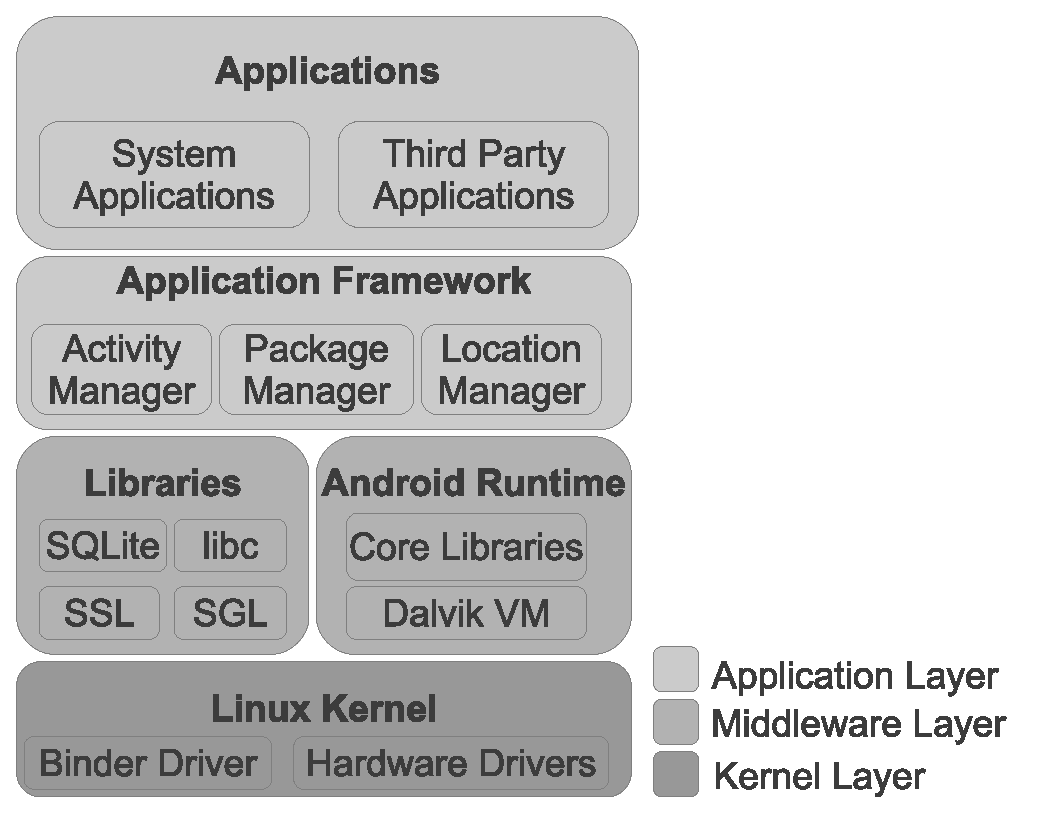
\psfig{file=android_arch.eps,width=2.0in}
\caption{Android Software Stack}
\label{fig:android}
\end{figure}

%The Linux-based kernel is located at the lowest layer of the 
%Android software stack. 
The kernel is responsible for providing 
the core functionality of Android, such as process management, 
networking, memory management, and device drivers to allow for 
the software to communicate with the hardware resources. 
Furthermore, the Linux kernel provides Android with the security 
functionality needed to enforce process isolation, hardware 
access privileges, and file access privileges through utilizing 
user identifiers (UIDs), group identifiers (GIDs) and file 
system access permissions.  
%Applications that are installed
%typically have a unique UID, however, Android also allows
%applications that are signed with the same signature to share
%a UID to allow two different applications to access each others
%resources (e.g., files).  However, since applications typically
%run in an isolated process under a unique UID, Android includes
%a mechanism in the Linux kernel (Binder) that allows
%inter-process communication.

%The middleware layer is located above the kernel layer of the 
%Android software stack, which 

The middleware consists of the native libraries 
and the runtime environment. The native libraries provide the 
system with machine independent functionality, such as the \textit{libc} 
library, a SSL implementation, and an SQLite implementation. 
The runtime environment consists of the core libraries and the 
Dalvik virtual machine. The core libraries provide the system 
with an implementation of the Java API, the Android libraries, 
and the Dalvik Virtual Machine's libraries. The Dalvik Virtual 
Machine is a process-level virtual machine that is responsible 
for executing Android applications that were compiled into 
Android's custom bytecode (DEX). 
%The middleware layer also 
%provides the system with a reference monitor that enforces 
%mandatory access control (MAC) for inter-component 
%communications.

%The application layer is located at the top of the Android 
%software stack and 
The application layer contains the application framework and 
applications. The application framework provides Android 
application developers with basic blocks with which 
applications directly interact.
%, such as the activity manager,
%package manager, location manager, and content providers.
%Applications are at the very top of the Android software stack
%and provides the user with software to perform specific tasks,
%such as a contact manager, a web browser, or a text messaging
%interface.  
Android applications are distributed as an application
package file (APK), which contains a manifest file that declares
the application's requested permissions and components, the DEX
bytecode of the application, resources, and application
certificates.  Applications may also define their own custom
permissions in the manifest file to enforce access control
policies on the components or data that they expose to other
applications.  Furthermore, applications may either be
\textit{system applications} (signed with the same signature
as the system image) or \textit{third-party applications}.

The access control policies of applications in the Android
system are achieved through the static installation-time
permission model, which are declared in the application's
manifest file and enforced by the reference monitor in the
middleware layer or by the Linux kernel.  
%An application's
%request to access sensitive data (e.g., a user's contacts)
%or hardware resources (e.g., the microphone, camera, etc.)
%must be granted by the user at the time of the application's
%installation.  Once the requested permissions are approved
%and the application is installed, the application will always
%be granted these permissions.

\subsection{Limitations of the Android Security Model}

While Android's permission-based security model suffices for
most applications, these static access controls can not address
the security requirements of applications targeted towards
the healthcare industry.

First, Android's current permission model does not support the
dynamic restriction of an application's privileges.  Since PHI
is not limited to medical records and images (e.g., MRI images),
but rather includes conversations between a doctor and a patient
during an appointment, malicious applications may exploit the
environment in which the mobile device is located to gather PHI
instead of attempting to steal data stored on the device.  For
example, a doctor may download a third-party voice memo recorder
to record reminders of non-sensitive information.  However, the
application may be malicious and launch a background service to
secretly record conversations that include details of PHI and
transmit the recorded audio to an external server.  Therefore,
a mechanism to dynamically restrict an application's privileges
is necessary to prevent the exposure of PHI by malicious
applications.

Second, Android's current framework also lacks the
system-level mechanism that is required to enforce security
policies on PHI data flows and revoke access to PHI.  Due to
the sensitivity of PHI, the system is required be able to
identify and revoke access to the PHI and enforce security policies
on the data (e.g., whether the PHI can be saved or forwarded).
On Android's current framework the organization loses
control the PHI once it is sent to the device, which is
unacceptable when dealing sensitive data.

\subsection{Addressing the Limitations of the Android Security Model}

%To address the limitations of Android's existing security model and
%the previously discussed security challenges for deploying mobile
%devices in the healthcare industry, 
DASF consists of three new
modifications to the Android platform. 

First, DASF provides a system-level mechanism for dynamically
enforcing system-wide privilege restrictions on applications.
Applications can programmatically impose dynamic system-wide privilege
restrictions on other applications if they request permission to
restrict a privilege.

Second, DASF utilizes dynamic taint tracking to identify sensitive
data and track the propagation of the sensitive data throughout
the system. To ease our implementation, this study utilizes
TaintDroid~\cite{taintdroid} to provide
the mechanism for tagging data and propagating the data's tag
throughout the system.  
%Further, we also leverage CleanOS'~\cite{Tang_osdi12} 
%extension of TaintDroid to provide the mechanism
%for revoking sensitive data.  
DASF uses the data's privacy
tags to enforce system-level security policies on the sensitive
data.  DASF augments these models by allowing
system-level security policies to be imposed on the data
(e.g., preventing the data from being saved or forwarded).

Third, we designed a application-layer message protocol at the
system-level that operates over an SSL connection to tag sensitive
data that is received from the server to allow the server to
impose system-level security policies on the data that it sends
to the device.  Further, our message protocol also allows the
server to dynamically impose system-wide privilege restrictions
on applications running on the device.

%Therefore, our contributions are providing system-level support for
%classifying sensitive data and enforcing security policies on that
%sensitive data, and allowing a server, or an application, to dynamically
%enforce system-wide privilege restrictions on the device.


\section{Security Framework Model}

%In this section, we begin by explaining the security policy model of
%DASF that we designed. Afterward, we focus on
%the architecture and implementation of the DASF prototype on Android.

%\subsection{Security Model}

On an Android device, there are
a set of applications, $A := \left\{a_{1},a_{2},\ldots,a_{n}\right\}$.
Each application, $\forall a_{i} \in A$, where $1 \le i \le n$,
contains a set of permissions that the application requests,
$P_{a_{i}} := \left\{p_{1}, p_{2},\ldots,p_{m}\right\}$,
and a set of components,
$C_{a_{i}} := \left\{c_{1},c_{2},\ldots,c_{q}\right\}$.
Each application is either a system application, $S_{A}$,
or a third-party application, $T_{A}$, such that $S_{A}\subset A$, and $T_{A} \subset A$,
but $S_{A} \cap T_{A} = \left\{\right\}$.

\subsection{Dynamic Privilege Restriction Security Policy.}  

A permission, $p$, is restricted if the restricted permission, denoted
as $R\left(p\right)$, is imposed
by a specific application $a_{i}$.
%such that $a_{j} \in A$ and $1 \le j \le m$.  
In Android, permissions are granted at the granularity
of the entire application.  If the permissions of a specific
application, $a_i$, is granted, its corresponding components,
$C_{a_i}$ are allowed to be launched. Obviously, for any application
that can successfully run, each of its components has to have the
permission to be launched. We use $L(C_{a_i})$ to
denote the launching of $a_i$'s components: $c_1, c_2,...,c_q$.
%
%Since permissions are granted at the granularity
%of the entire application rather than at the granularity of its individual
%components, the application's components that are permitted
%to be launched is denoted as $L\left(C_{a_{i}}\right)$. This means,
%$\forall c_{k} \in C_{a_{i}} : L\left(c_{k}\right)$ such that 
%$1 \le k \le o$.  
Furthermore, we denote killing the process
that an application, $a_{i}$, is running under as $K(a_{i})$.

Therefore, the security policy for an application is a procedure of
imposing the restricted permissions which determine whether or not the
application and its components can be launched. Given an application
$a_i$, its components launching, $L(C_{a_i})$, will be
successful as long as one the security policy satisfy any one of the
following conditions:

\[\left\{
\begin{array}{l}
a_i \in S_A\\
%a_i \in T_A \wedge R\left(p\right) \wedge p \in P_{a_{i}} \\
%\wedge a_i = a_j\\
a_i \in T_{A} \wedge \lnot R\left(p\right) \wedge p \in P_{a_{i}}.\\
\end{array}
\right.
\]


%for starting an application, $a_{i}$,
%and it's components, $C_{a_{i}}$, is defined as follows.

%$a_{i} \in S_{A} \to L\left(C_{a_{i}}\right)$

%$a_{i} \in T_{A} \wedge R\left(p\right) \wedge p \in P_{a_{i}} \wedge a_{i} = a_{j} \to L\left(C_{a_{i}}\right)$

%$a_{i} \in T_{A} \wedge \lnot R\left(p\right) \wedge p \in P_{a_{i}} \to L\left(C_{a_{i}}\right)$

\begin{comment}
$a_{i} \in T_{A} \wedge R\left(p\right) \wedge p \in P_{a_{i}} \wedge a_{i} \neq a_{j} \to \lnot L\left(C_{a_{i}}\right)$
\end{comment}
More significantly, DASF is able to impose the
policy on application that are already running when a permission is
dynamically restricted for a security purpose.  In that case, any
running application $a_i$ with the following updated policy:
\[\left.
\begin{array}{l}
(a_{i} \in T_{A}) \wedge R\left(p\right) \wedge (p \in P_{a_{i}})\\
\end{array}
\right.
\]
will lead to $K(a_i)$, i.e., be terminated.  And the running
application status with the following
new policy, $ a_{i} \in T_{A} \wedge \lnot R\left(p\right) \wedge p \in P_{a_{i}}$,
%\[\left \{
%\begin{array}{l}
%a_{i} \in S_{A}\\
%a_{i} \in T_{A} \wedge \lnot R\left(p\right) \wedge p \in P_{a_{i}} \wedge a_{i} = a_{j}\\
%\end{array}
%\right.
%\]
will become $\lnot K(a_i)$, i.e., not be affected.
%Moreover, the security policy imposed on applications that are 
%already running when a permission is dynamically restricted
%is defined as follows.

%$a_{i} \in S_{A} \to \lnot K\left(a_{i}\right)$

%$a_{i} \in T_{A} \wedge \lnot R\left(p\right) \wedge p \in P_{a_{i}} \wedge a_{i} = a_{j} \to \lnot K\left(a_{i}\right)$


%$a_{i} \in T_{A} \wedge R\left(p\right) \wedge p \in P_{a_{i}} \to K\left(a_{i}\right)$

In other words, an application's components are always allowed to
start if they belong to a system application.  Moreover, system
applications are never forcibly closed if a permission is dynamically
restricted.  If the application is a third-party application, however,
the following policies are enforced. First, a third-party
application's components are not permitted to start if the application
requests a permission that is currently restricted and the application
is not the one that imposed the permission restriction.  Second, a
third-party application's components are permitted to start if the
application does not request any permissions that are currently
restricted. Furthermore, if a permission is dynamically restricted and
a third-party application that is currently running has requested that 
permission and was not the application that imposed the permission
restriction, the application will be forcibly closed.

%Since DASF provides support for a certified~\footnote{The
%  certification process can be dictated by the organization, e.g., a
%  hospital, throught an out-of-band channel.} third-party
%applications to programmatically restrict permissions, the
%application, $a_{i}$, must define a set of permissions that it is
%permitted to restrict, $X_{a_i} := {p_1, p_2,\ldots,p_m}$,
%during the application's installation and approved by the user to prevent
%the abuse of dynamic permission restrictions.  Thus, a third-party application,
%$a_{i}$, is allowed to restrict a permission, $p$, if $p \in X_{a_{i}}$.

\subsection{Security Policies on Sensitive Data.}
A mobile device contains a set of data (e.g., strings, integers, arrays,
etc.) in RAM, $\left\{d_{1},d_{2},\ldots,d_{n}\right\}$,
each of which has its corresponding sensitivity level. In our
framework, we use a privacy tag, $T(d_i)$, with the possible values of
$\left\{t_{1},t_{2},\ldots,t_{m}\right\}$, to represent data $d_i$'s
sensitivity level.
%$\left\{t_{1},t_{2},\ldots,t_{m}\right\}$, to represent a variety of 
%sensitivity levels.  
%privacy tag: $T(d_i)$, where $1\leq i\leq n$. 
%Since we utilize the dynamic taint tracking system provided
%by TaintDroid, each element in the set of data also includes
%a privacy tag, $T\left(d_{i}\right)$, which denotes the data's sensitivity level
%that comes from the set of possible privacy tags,
%$\left\{t_{1},t_{2},\ldots,t_{m}\right\}$.
%%
%
%Thus, we denote the set of data in the Java stack as a set
Thus, we can denote the data set as a set containing a privacy tag and
the data:
%containing a privacy tag and the data,
$D := \left\{\left\{d_{1}, T\left(d_{1}\right)\right\},\left\{d_{2},T\left(d_{2}\right)\right\},\ldots,\left\{d_{n},T\left(d_{n}\right)\right\}\right\}$.

It is possible for two pieces of data, $d_{j}$, $d_{k}$, where $1 \le
j \le n$ and $1 \le k \le n$,  with different privacy tags
to be combined (e.g., concatenating two strings with different
sensitivity levels).  The general propagation rules of the
privacy tags are as follows when data with two different privacy tags
are combined:

$T(d_{j}) \ge T(d_{k}) \to T(d_{j}\wedge d_{k}) = T(d_{j})$,

$T(d_{j}) < T(d_{k}) \to T(d_{j} \wedge d_{k}) = T(d_{k})$.

These propagation rules ensure that when two pieces of
data are combined, the highest sensitivity level is propagated
to the combined data.   This means that if the sensitivity
level of $d_{j}$ is greater than or equal to the sensitivity
level of $d_{k}$, the combined data has the sensitivity level
of $d_{j}$.  Further, if the sensitivity level of $d_{j}$ is
less than the sensitivity level of $d_{k}$, the combined data
has the sensitivity level of $d_{k}$.

We define two operations on the data that our security policy
must handle.  First, $W(d_{j})$, denotes writing the data to
flash memory (e.g., to a file or an SQLite database). Second,
$F(d_{j})$ denotes forwarding the data from the device
(e.g., through a socket, bluetooth socket, SMS, and MMS).
Furthermore, data, $d_{j}$, that can either be forwarded from the
device or written to flash memory is denoted as $FW\left(d_{j}\right)$.
The operations that are permitted on the data are determined by the
data's privacy tag.  The privacy tag, $t_0$, denotes
that $T(d_{j}) = t_0 \to \lnot FW\left(d_{j}\right)$. The privacy tag,
$t_1$, denotes $T(d_{j}) = t_1\lnot W\left(d_{j}\right)$.  Finally,
the privacy tag, $t_2$, denotes 
$T(d_{j}) = t_2 \to \lnot F\left(d_{j}\right)$.  Furthermore, we reserve
the privacy tag, $t_m$, to denote sensitive information that have
no security policies enforced by the system.  The value of $m$ is a
system parameter and can be adjusted depending on the requirement of
the security levels. 

To ensure that the security policies are enforced correctly when
combining two pieces of data with different sensitivity levels,
the propagation rules of the data's sensitivity levels must
include an escalation of sensitivity levels.  For example, if
data with the privacy tag $t_1$ is combined with data with
the privacy tag $t_2$, the combined data should have the
privacy tag $t_0$ rather than $t_1$ or $t_2$.  Thus, the propagation
of privacy tags are adjusted as follows when data is combined:

$T\left(d_{j}\right) = t_1 \wedge T\left(d_{k}\right) = t_2 \to T\left(d_{j}+d_{k}\right) = t_0$.

This propagation rules ensures that if data that is restricted from
being forwarded from the device is combined with data the is restricted
from being written to flash memory, the combined data will be restricted
from being written to the flash memory and forwarded from the device.

\subsection{Application-Layer Message Protocol.}   
DASF also includes an application-layer message protocol
that allows a server to dynamically enforce privilege restrictions
on the device and enforce the previously mentioned security policies
on data that is sent to the device.  The message
protocol assumes that it is built over an SSL connection to ensure
a secure communication channel between the client (e.g., mobile
device) and the server.

The message protocol consists of applications sending a request to
the server (e.g., requesting data) and the server responding back
to the request (e.g., sending the data).  The message protocol
allows the server to impose a sensitivity level on the data in
its response, and thus, impose a security policy on the data that
it sends to the client.  We call the server responding to the
client's request for data as a \textit{data message}.
The header of the \textit{data message} denotes the type of message,
sensitivity level, and the length of the payload.  The contents of a
\textit{data message} is shown in Fig.~\ref{fig:datamessage}.

\begin{figure}[ht]
\centering
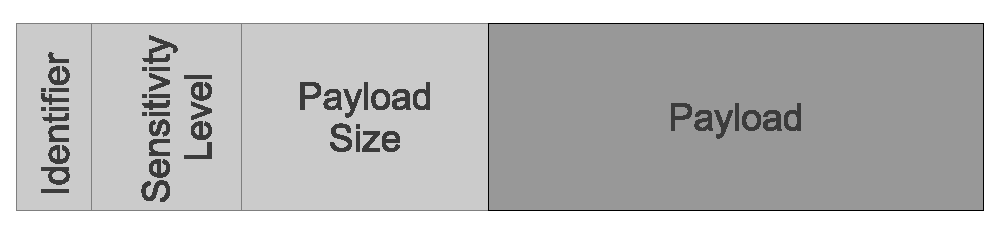
\psfig{file=data_message.eps, width=2.5in}
\caption{Data Message}
\label{fig:datamessage}
\end{figure}

%\vspace{-3mm}

When an application requests data from the server, the server
responds back to the client with
$data\_message\left(\left\{sensitivity\_level, response\right\}\right)$.
The system extracts sensitivity level and applies that sensitivity level
to the response before passing it to the application.  The sensitivity
level, $s$, corresponds to one of the four privacy tags that we previously defined.
For example,  $s \in \left\{t_m,..., t_2, t_1, t_0\right\}$.

The server can also dynamically impose any privilege restrictions on
the device without asking the user for permission.  To prevent the
abuse of server-imposed privilege restrictions, the application must
be declared as a \textit{medical application} during its installation
and the system insures that the client application connects to the
organization's trusted server. The above assurance is achieved by a
server-side periodic encrypted heartbeat message that confirms the
application's aliveness.  Note that under our security framework, the
connection between the server and the \textit{medical application} is
supposed to be persistent; the tear-down of the connection will lead
to the termination of the application due to the security concern. 
The system secret key update and the privilege control message
(as described below) can be arranged as a piggyback in the heartbeat 
messages.  
%The server may dynamically impose
%privilege restrictions, or unrestricted previously imposed privilege
%restrictions, on the device by prepending a
%\textit{privilege control message} to the \textit{data message}.

The dynamic security provisioning is enforced by the \textit{privilege
  control message}, which must be encrypted with a one-time key so
that DASF can verify that the policy originated from the server and to
prevent replay attacks. The one-time key can be provided by a server
generated one-way key chain, similar to S/Key mechanism~\cite{skey}. 
Our security framework fetches the initial master secret key from the
server when the device is first booted and updates the master key, if
necessary, through the server heartbeat message as described above. 
%
%Furthermore, the payload of the \textit{privilege control message} must be
%encrypted using a one-time key to prevent applications from abusing
%this functionality.  The payload must be encrypted with a one-time
%key so that DASF can verify that the policy
%originated from the server and to prevent replay attacks.  Our
%security framework fetches the initial secret key from the server
%when the device is first booted.
%
%The payload of the \textit{privilege control message} contains a list
%of privilege restrictions, privilege unrestrictions, and a new secret
%key.  
%The entire payload is encrypted using the previous key,
%$E\left(key, payload\right)$.  
The header of the \textit{privilege control
 message} contains the type of message, a flag denoting that a data message
is appended, and the length of the payload. The contents of 
a \textit{privilege control message} is shown in
Fig.~\ref{fig:privilegemessage}.  When the system receives a
\textit{privilege control message}, it passes the payload to DASF.
If the security framework successfully decrypts
the payload, $D\left(key, payload\right)$, the set of permission restrictions
and unrestrictions are imposed and the secret key is updated.

\begin{figure}[ht]
\centering
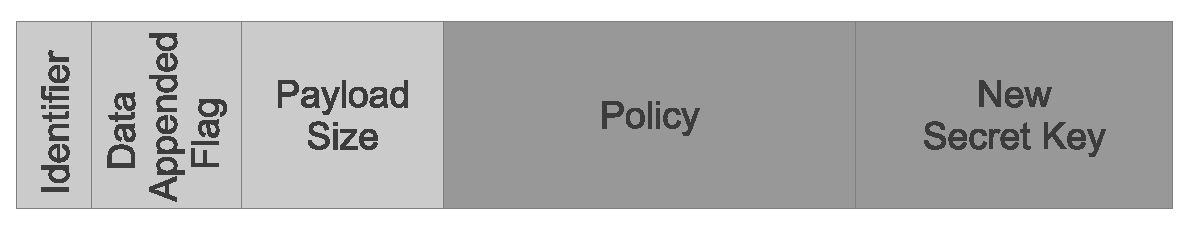
\psfig{file=policy_message.eps, width=2.5in}
\caption{Privilege Control Message}
\label{fig:privilegemessage}
\end{figure}


\vspace{-3mm}
\section{Evaluation}

We tested our prototype of DASF on a Galaxy Nexus (\textit{GT-I9250}),
which includes a 1.2 GHz dual-core ARM Cortex-A9 processor,
1 GB of RAM, and 16 GB of flash memory.  Our goal is to
illustrate that DASF provides adequate protection against the
previously discussed security threats and provides a reasonable
performance overhead.

\subsection{Security Threat Evaluation}

As previously discussed, we consider four different types of security
threats that DASF must provide protections against
\textit{(1) legitimate user misbehavior},
\textit{(2) malicious users}, \textit{(3) application misbehavior},
and \textit{(4) malicious applications}.  Since CleanOS addresses
the 2nd security threat by providing a mechanism for revoking sensitive
data and we assumed that our model was built on top of CleanOS, we do not
evaluate that security threat.  However, we perform the following three
tests to show that DASF adequately addresses the remaining
security threats.

\begin{itemize}
\item \textit{Legitimate user misbehavior.}  We created an application that receives
  data from the server that has restrictions imposed on the data.  Next, we
  attempt to manually save and forward the data by passing it to other
  applications on the device that attempt to perform these operations.
\item \textit{Application misbehavior.}  We created an application that requests
  data from the server (e.g., an MRI image) that is restricted to be saved
  to the device.  When the application is receiving the data, it attempts
  to break the policy by writing the data directly to a file when receiving
  it.
\item \textit{Malicious applications.}  We created a malicious voice memo recorder
  application that attempts to steal information from the environment. Our
  voice memo recorder requests the \textit{record audio} permission
  and the \textit{internet} permission to allow users to sync memos to their
  other devices.  However, the voice memo recorder maliciously launches
  a background service to secretly record audio in the background and
  transmits the recorded audio to an external server.
\end{itemize}

We ran the first test and confirmed that DASF successfully
blocked the data from being forwarded from the device and saved to the device.
Thus, DASF enforced the policy imposed on the data from the
server.

When we ran the second test, we confirmed that DASF
successfully blocked the data from being saved to a file.  Moreover, we
modified the application to check the sensitivity level on the data
received and determine whether to store the data in a file or keep it
in main memory.

Finally, we ran the third test by starting the malicious
voice memo recorder and confirmed that it successfully recorded data in the
background.  Next, we created another application that restricts the
\textit{record audio} permission when the user presses a button.  DASF
successfully closed the malicious voice memo recorder, including its
background service, and prevented it from being opened again until
the \textit{record audio} permission was unrestricted.  Instead of
restricting the permission by pressing a button, an application can
be designed to restrict permissions when certain RFID tags are
scanned, which would allow doctors to simply wave their device by
an RFID tag when entering areas where conversations may include
PHI data (e.g., outside of patient rooms).  To prevent malicious
applications from attempting to steal sensitive information stored on
the device (e.g., PHI information authorized to be saved to the device),
we rely on Android's file system privileges (e.g., UIDs) and our restriction
that medical applications are assigned a unique UID.  

\vspace{-3mm}
\subsection{Performance Evaluation}

Since DASF is invoked whenever an application, or application
component is started, we tested the performance overhead on the starting
activities and services on the Galaxy Nexus running our prototype.  To get
a baseline for comparison, we repeated the tests on the stock Android \textit{Jelly Bean}
platform and on TaintDroid.  Furthermore, we also tested the overhead of
\textit{medical applications} using our message protocol.

\textbf{Application Component Overhead.}  Whenever an activity or service is
started, our\textit{Privilege Restriction Service} is invoked to determine
whether the activity or service may be started.  Therefore, we tested
the time that it takes to launch activities and service.  We repeated
the same tests on the stock Android \textit{Jelly Bean} platform and on TaintDroid.

Fig.~\ref{fig:component} shows the performance overhead of starting activities and services on
our prototype, the stock Android \textit{Jelly Bean} platform, and on TaintDroid.
As the figure shows, our prototype took 118 milliseconds on average to
start an activity and 17 milliseconds on average to start a service.  The
stock Android \textit{Jelly Bean} platform took 94 milliseconds on average
to start an activity and 8 milliseconds on average to start a service.  The
TaintDroid platform took 115 milliseconds on average to start an activity
and 14 milliseconds on average to start a service.  We assume that the
overhead when comparing TaintDroid and the stock Android \textit{Jelly Bean}
platform is due to the extra memory that needs to be allocated for the 
taint tags in the Java stack.  When compared to the overhead of TaintDroid,
using our prototype results in a minimal overhead on starting activities and services.

\begin{figure}[ht]
\centering
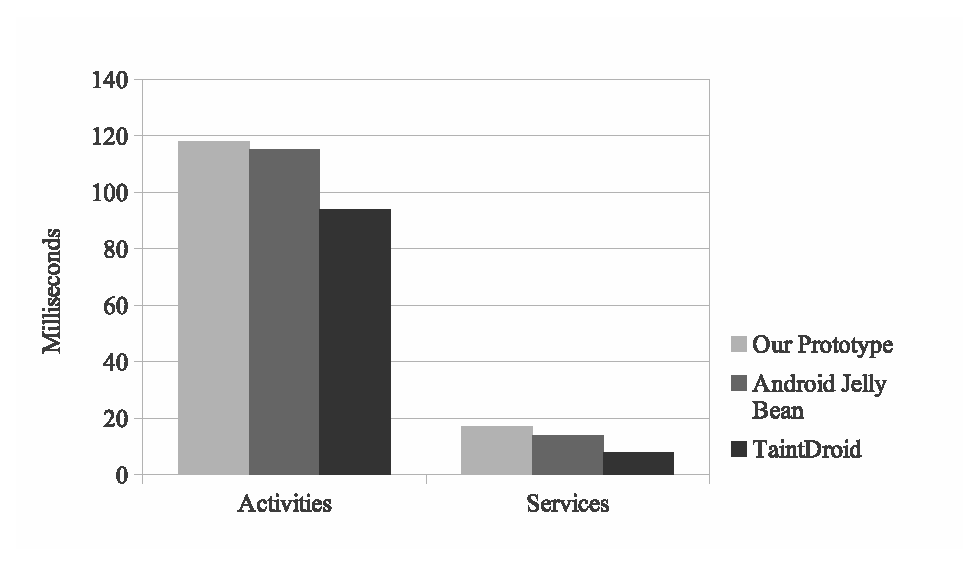
\psfig{file=component_performance.eps, width=2.6in}
\caption{Performance overhead when starting activities and services}
\label{fig:component}
\end{figure}

\textbf{Message Protocol Overhead.}  To test the overhead of our message protocol,
we created an application that requested data of varying length from the server.
The data lengths that we tested are 1-KB, 5-KB, 100-KB, 1-MB, 5-MB, and 50-MB.
We have recorded the time that it took the \textit{MessageInputStream} to receive
the message and pass the data back to the application.  We disregarded the time
that it took to transmit the data over the network since that is related
to the overhead of the network speed rather than the overhead caused by
our message protocol.  Furthermore, we also recorded the time that it
took the system to enforce policy restrictions and unrestrictions.

As the Fig.~\ref{fig:performance} suggests, our message
protocol took 54931 nanoseconds on average to parse and return 1-KB of
data back to the application, 73242 nanoseconds on average for 5-KB, 
720215 nanoseconds on average for 100-KB, 8 milliseconds on average
for 1-MB, 49 milliseconds on average for 5-MB, and 468 milliseconds
on average for 50-MB.  Furthermore, it took 81 milliseconds on average
to impose permission restrictions and around 2 milliseconds on average
for permission unrestrictions.

\begin{figure}[ht]
\centering
\subfigure[Data Message Overhead]{
	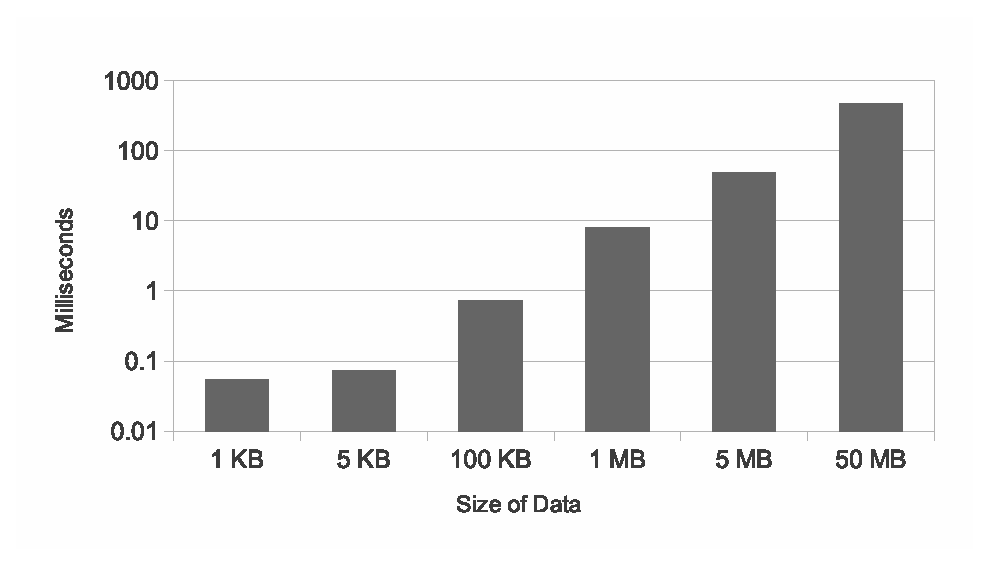
\psfig{file=kb_performance.eps, width=2.6in}
	\label{fig:kbperformance}
}
\subfigure[Privilege Control Message Overhead]{
	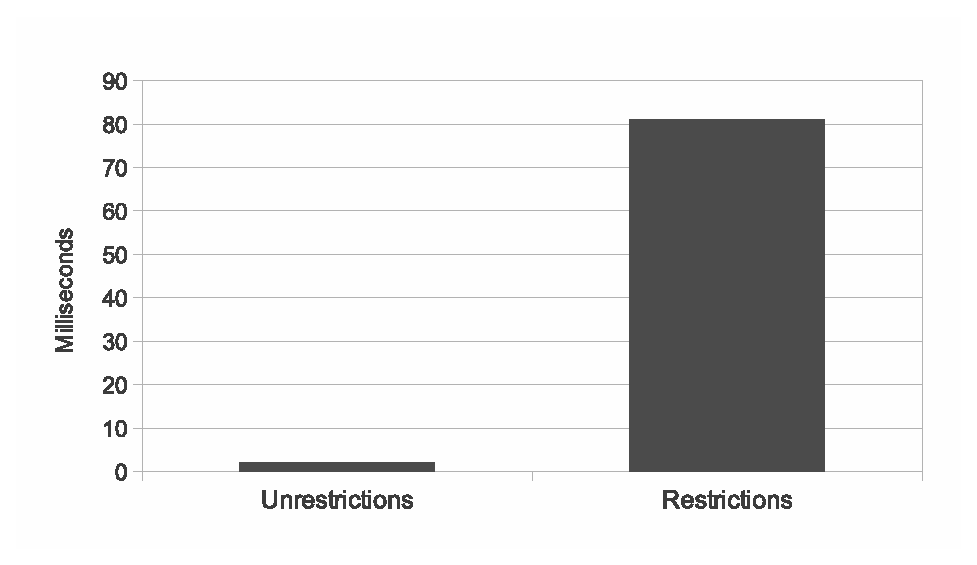
\psfig{file=policy_performance.eps, width=2.4in}
	\label{fig:policyperformance}
}
\caption{Message Protocol Performance Overhead}
\label{fig:performance}
\end{figure}

\subsection{Limitations}

There are three current limitations of the DASF prototype.  First,
the sensitivity level of the data can be cleared since TaintDroid's
taint propagation logic does not address implicit flows. This is a major
concern because applications can clear the sensitivity
level from data and break the security policies imposed on that data.
Second, TaintDroid also does not allow applications to use third-party
native libraries since they can be used to clear privacy tags.  Third,
DASF does not currently handle propagating
the sensitivity level of data displayed on the screen.  Therefore,
a user can break the security policy on sensitive data by taking a
screenshot of an image.


\section{Related Work}
It is believed that 1.4 billion smartphones will be in active by the
end of 2013~\cite{rbiresearch}, and 57\% of them will run the Android
operating system. The popularity of the Android devices has made it
the top target of the mobile malware~\cite{Felt,Becher,xjiang_oak12}
and other potential attacks~\cite{Fahl,hijack}. To improve the
smartphone security defense, a number of Android system extensions
\cite{Nauman,Beresford,xjiang_11,Hornyack,Ongtang,Enck_ccs09,Lange,Andrus}
have been proposed. Apex~\cite{Nauman} proposes an Android enforcement
frame that enables flexible permission granting and resource
restrictions.  MockDroid~\cite{Beresford} is closely related to this
work in that the Android system is modified to protect the privacy.
The main difference, however, is that MockDroid protects the privacy
by adding perturbations to achieve ambiguity.  Our framework
offers a system-wide, dynamic and strict access restrictions to
protect the sensitive data.  In addition, our framework is 100\%
transparent to general Android applications.  TISSA~\cite{xjiang_11}
protects the private information leakage by an extra permission
layer. AppFence~\cite{Hornyack} provides a similar fine-grained
permission control.  Different from their schemes, our security
framework is more versatile, protecting both outgoing and 
incoming data through an on-demand dynamic security provisioning.
Saint~\cite{Ongtang} uses the design-time security policies to manage 
permissions. Kirin~\cite{Enck_ccs09} proposes a set of security rules
to mitigate malware.  L4Android~\cite{Lange} and Cells~\cite{Andrus}
provide the improved OS isolation for security.  

%TaintDroid~\cite{taintdroid} provides a information flow monitoring
%system to detect the potential privacy leakage. This idea is adopted
%in our system framework to enforce the data access privilege and
%propogation restrictions.

TaintDroid~\cite{taintdroid} provides a information flow monitoring
system to detect the potential privacy leakage. This idea is adopted
in our system framework to enforce the data access privilege control
and propagation restrictions.
Static analysis has been used to detect privacy leak in Android
applications~\cite{Batyuk} and potential security
vulnerabilities~\cite{Lu_ccs12}.  Crowdroid~\cite{Burguera} analyzes
the system calls dynamically to detect the malware.  Android
permission specification has been thoroughly studied in
Stowaway~\cite{Felt_ccs11} and PScout~\cite{Au_ccs12}.  As discussed
previously, the permission based Android security system is
insufficient to address the security challenges in the application
compliant with the HIPAA rule.


%\vspace{-3mm}
\section{Conclusion}

This paper describes a distributed security framework (DASF) for
Android-based mobile operating systems designed to provide dynamic
privilege restrictions on applications and security policies on
sensitive data sent to the device.  Unlike Android's current security
model, DASF allows an application's permissions to be restricted
dynamically to address the security concerns of mobile devices being
used in sensitive environments.  Further, DASF also allows the
organization to remain in control of the sensitive data that it sends
to the mobile device by imposing security policies on that data.  We
implement a prototype of DASF by creating a system service to enforce
privilege restrictions on applications, and our experiments show that
DASF addresses the limitations of Android's current security model
while imposing a reasonable performance overhead. 


% Our future work
%includes the system enhancement in the following aspects.  First, we need to
%develop a mechanism to differentiate the network brokeage and security
%attacks.  Ideally, our DASF will allow a short disconnect operation without
%sacrificing the security countermeasure capabilities. Second, we will start
%our development of DASF on a native Android system instead of the TaintDroid
%to further improve the system latency performance and enhance the security
%performance as discussed previously.  



%a custom \textit{InputStream} to 
%handle our message protocol, and by
%placing hooks in the Android system to enforce
%the security policies.  Further, we built a server
%module to send data and security policies to
%the device to demonstrate that the security
%policies can be dynamically imposed on both
%an application's privileges and on sensitive
%data.  Our experiments shows that DASF
%addresses the limitations of
%Android's current security model while
%imposing an reasonable performance overhead.

\bibliographystyle{plain}
\bibliography{ref}
%\end{scriptsize}


\end{document}
